\documentclass[a4paper, 12pt]{article}
\usepackage[T1]{fontenc}
\usepackage{lmodern}
\usepackage{color}
\usepackage{amsfonts}
\usepackage{epstopdf}
\usepackage{matlab}
%\documentclass{book}
\usepackage{blindtext}
\usepackage{hyperref}
\usepackage[brazil]{babel}
\usepackage{amssymb}
\usepackage[utf8]{inputenc}
\usepackage{amsmath}
\usepackage{indentfirst}
\usepackage{graphicx}
\usepackage{multicol,lipsum}
\usepackage[a4paper,
top=3cm, left=3cm, bottom=3cm, right=3cm]{geometry}
\usepackage{setspace}
\usepackage{multirow}
\usepackage{float}
\usepackage[table]{xcolor}
%\usepackage{pdflscape}
\usepackage[DIV=15]{typearea}
\usepackage[nottoc]{tocbibind}
\usepackage[sort,numbers]{natbib}
%\usepackage{cite}
\usepackage{matlab}


\documentclass[letterpaper]{article}
% bib pack %%%%%%%%%%%%%%%%%%%%%%%%%%%%%%%%%%%%%%%%%%%%%%%%%%%%%%%%%%%%%%%%%%%%%
\usepackage[utf8]{inputenc}
\usepackage{geometry}
    \geometry{left=3cm,right=2cm,top=2cm,bottom=2cm}
%
\usepackage[spanish]{babel}
%
\usepackage[fixlanguage]{babelbib}
    \bibliographystyle{babunsrt}
%
\usepackage{url}

\begin{document}
%\maketitle

\begin{titlepage}
	\begin{center}
		

\vspace{10pt}
%\begin{figure}[!ht]
%\centering
%
\includegraphics{puc-rio-logo.png}

%\end{figure}
\begin{figure}[!ht]
\centering

\includegraphics{images/puc-rio-logo.png}
\end{figure}
\huge{Controles e Servomecanismos}
        \vspace{70pt}
        
		\textbf{ENG1407}
		\textbf{\large{\\ }}
		
		\vspace{30pt}
		\textbf{\small{\\Lista 8 - Problema nº 2}}
		\vspace{75pt}
		
	\end{center}
	
	\begin{flushleft}
		\begin{tabbing}
			Aluno(a)\qquad\qquad\=\>Gabriel Novaes Pereira - 1813157\\ \>Paloma Fernanda Loureiro Sette - 1621595\\
			
			Professor(a)\>Ana Pavani e Vivian Suzano Medeiros\\
	\end{tabbing}
		  
	\end{flushleft}
	\begin{center}
		%\vspace{\fill}
		\vspace{90pt}
		Rio de Janeiro, 07 de Junho de 2022
	\end{center}
\end{titlepage}
%%%%%%%%%%%%%%%%%%%%%%%%%%%%%%%%%%%%%%%%%%%%%%%%%%%%%%%%%%%
\newpage
\tableofcontents
\thispagestyle{empty}

\newpage
\pagenumbering{arabic}

\newpage

%\newcommand{\listequationsname}{Lista de Equações}
%\newlistof{myequations}{equ}{\listequationsname}
%\newcommand{\myequations}[1]{%
%\addcontentsline{equ}{myequations}{\protect\numberline{\theequation}#1}\par}

%\listofmyequations
\newpage


\newpage

\listoffigures
\thispagestyle{empty}

\newpage
%%%%%%%%%%%%%%%%%%%%%%%%%%%%%%%%%%%%%%%%%%%%%%%%%%%%%%%%%
%%%%%%%%%%%%%%%%%%%%%%%%%%%%%%%%%%%%%%%%%%%%%%%%%%%

\section{Introdução}
Este trabalho tem como objetivo apresentar as soluções referentes ao problema de número 2, da lista 8 de soluções discursivas da disciplina de Controles e Servomecanismos. 

Como sabemos, a determinação da existência ou de um certo tipo de característica de estabilidade em um sistema linear e invariante é reduzido à determinação da localização de raízes de polinômios.


\section{Problema 2}
Pede-se que consideremos o SLIT-TC modelado pelo seguinte diagrama em blocos:

\begin{figure}[H]
\centering
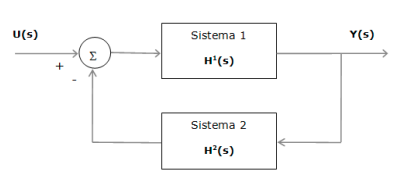
\includegraphics[scale = 0.7]{images/diagrama-blocos.png}
\label{filtro1}
\caption{Diagarama de blocos do problema nº 2}
\end{figure}

Cujas funções de transferência se dão por:

\begin{equation}
    H^1(s) = \frac{K(s+5)}{s^2+6s+13}
\end{equation}

\begin{equation}
    H^2(s) = \frac{1}{s^2+4s+5}
\end{equation}



\subsection{Parte 1}
O método do lugar das raízes irá se basear na equação seguinte:

\begin{equation}\label{eq:primary}
    F(s) = (s^2+6s+13)(s^2+4s+5)+K(s+5) = 0
\end{equation}

Onde $K$ é o parâmetro que varia e que, ao variar, modifica os coeficientes da equação e, consequentemente, suas raízes.

Sabemos que podemos identificar três categorias para o Lugar das Raízes (\textit{Root Locus}):

\begin{itemize}
    \item Lugares das Raízes - onde as raízes ocupam quando $K$ variam em $[0, \infty]$.
    \item Lugares complementares das Raízes - onde as raízes ocupam quando $K$ varia em $(-\infty, 0]$ 
    \item Contorno das Raízes - local que as raízes ocupam quando a equação (\ref{eq:primary}) possui mais de um parâmetro variável. 
    \item Lugares Completos das Raízes - Local que as raízes ocupam quando, existindo um único parâmetro variável, $K$ varia no intervalo $(−\infty, \infty)$ . 
\end{itemize}


para a primeira parte deste problema, pede-se que determinemos as características do Gráfico do Lugar das Raízes ($K\geq0$).
\begin{equation}\label{eq: exp_root_locus}
    \frac{(s+5)}{(s^2+6s+13)(s^2+4s+5)}=\frac{-1}{K}
\end{equation}

A expressão (\ref{eq: exp_root_locus}) será usada para apresentar o conceito de Lugares das Raízes.



\subsubsection{Pontos com K = 0 (Partida do traçado)}

Os pontos nos quais $K=0$ são bem determinados no gráfico e, de acordo com o Teorema, \textbf{são os pólos} de $H^1(s)H^2(s)$. O pólos levam o quociente a valer infinito, logo, serão os valores de s que levarão o denominador a zero.

\begin{equation}
    (s^2+6s+13)(s^2+4s+5)=0
\end{equation}

Resolvendo a expressão quadrática do primeiro parênteses para encontrar suas raízes, chegamos ao seguinte resultado:
\begin{equation}\label{eq:polos1}
    p_{0}=-3 +2i; \quad     p_{1}=-3 -2i;
\end{equation}

Analogamente, para a segunda expressão, temos:
\begin{equation}\label{eq:polos2}
    p_{2}=-2 +i; \quad p_{3}=-2 -i.
\end{equation}

Portanto, os pólos são identificados por $p_{0}$, $p_{1}$, $p_{2}$ e $p_{3}$. \blacksquare



\subsubsection{Pontos com K=\infty}

De acordo com o Teorema, os pontos de $K = \infty$ dos Lugares Completos das Raízes \textbf{são os zeros} de $H^1(s)H^2(s)$. Os \textit{zeros} levam o quociente a valer zero, logo, serão os \textbf{valores de $s$ que levarão o numerador a zero}. Portanto,

\begin{equation}
    (s+5)=0
\end{equation}
\begin{equation}
      z_{0}=-5; \quad  z_{1} = \infty; \quad z_{2}=\infty; \quad z_{3} = \infty
\end{equation}

Logo, $z_{1}$, $z_{2}$ e $z_{3}$ levam a função a zero por tornar o denominador infinito. \blacksquare



\subsubsection{Número de Ramos} 
Um ramo dos Lugares das Raízes Completos é a trajetória descrita por uma das raízes quando $K$ varia de $-\infty$ a $\infty$. Desta maneira, o \textbf{número de ramos dos Lugar das Raízes Completos é o número de raízes da equação}. \\

Ou seja, de acordo com o Teorema, o número de ramos dos Lugares das Raízes Completos é dado pelo maior entre $m$ e $n$. 

Portanto, inspecionando a equação (\ref{eq:primary}), temos que:

 \begin{equation}
    N_{r}= maior\quad entre\quad n\quad e\quad m
\end{equation}

Sendo $n = 4$ e $m = 1$. Logo, 

\begin{equation}
    N_{r}= 4 \quad \blacksquare
\end{equation}


\subsubsection{Assíntotas do Gráfico dos Lugares Completos das Raízes} 

Ramos que tendem a $\infty$ quando $K \longrightarrow$ \infty.

\paragraph{Número de Assíntotas} - 
As propriedades dos lugares completos das raízes nas proximidades do infinito são importantes, já que, quando $n \neq m$, teremos que $2|n-m|$ irão tender a $\infty$ no plano complexo $S$. \\

Então, o número de assíntotas para $K \geq 0$ e $K \leq 0$ é:
\begin{equation}
    N_{a}=2|n-m| = 2|4-1| \quad \longrightarrow \quad N_{a} = 6 \quad \blacksquare
\end{equation} 
Assim, serão 6 assíntotas, 3 nos Lugares e 3 nos Lugares Complementares das Raízes.

\paragraph{Ângulos das assíntotas} - 
Os Lugares das Raízes, para $K \geq 0$, são assintóticos a linhas retas com ângulos dados por 

\begin{equation}
    \theta_{\alpha} = \frac{(2_{\alpha}+1)\pi}{n-m} \quad \longrightarrow \quad \theta_{\alpha} = \frac{(2_{\alpha}+1)\pi}{3}  
\end{equation}

Para $K \leq 0$, os lugares completos das raízes terão ângulos de assíntotas dados por

\begin{equation}
    \theta_{\alpha} = \frac{2_{\alpha}\pi}{n-m} \quad \longrightarrow \quad \theta_{\alpha} = \frac{2_{\alpha}\pi}{3}  
\end{equation}

Onde $\alpha \in [0, |4-1| - 1]$ e $n = 4$ e $m = 1$ são os graus dos polinômios em (\ref{eq:primary}).\\

Portanto, os ângulos serão:

\begin{equation}
	\theta_{\alpha} = \frac{(2_{\alpha}+1)\pi}{3}  \quad \therefore \quad \theta_{0}=\frac{\pi}{3}; \quad \theta_{1}=\pi; \quad \theta_{2}=\frac{5 \pi}{3} . \quad \blacksquare
\end{equation}


\begin{equation}
	\theta_{\alpha} = \frac{2_{\alpha}\pi}{3} \quad \therefore \quad \theta_{0} = 0; \quad \theta_{1}=\frac{2 \pi}{3}; \quad \theta_{2} = \frac{4 \pi}{3} . \quad \blacksquare
\end{equation}


\paragraph{Interseção das Assíntotas}

\begin{enumerate}
    \item A interseção das 6 assíntotas ocorre sobre o eixo real;
    \item A interseção acontece em
    
    \begin{equation}
    \sigma = \frac{b_{1}-a_{1}}{n-m}    
    \end{equation} 
    Onde $a$, $b$, $n$ e $m$ são parte da equação (\ref{eq:primary}).
\end{enumerate}

\begin{equation}
		\sigma = \frac{\Sigma \Re pn  - \Sigma \Re zn}{n-m}
\end{equation}\begin{equation}
	\sigma =\frac{-5}{3} \quad \blacksquare
\end{equation}



\subsubsection{Lugares Sobre o Eixo Real} 
É interessante lembrarmos que, de acordo com o Teorema:

\begin{enumerate}
    \item Os Lugares das Raízes, i.e., para $K \geq 0$, só podem ser encontrados em uma dada seção do eixo real se o número total de pólos e zeros de $H^1(s)H^2(s)$, à direita da seção, for ímpar;
    \item Os Lugares das Raízes, i.e., para $K \leq 0$, só podem ser encontrados em uma dada seção do eixo real se o número total de pólos e zeros de $H^1(s)H^2(s)$, à direita da seção, for par.
\end{enumerate}

Portanto, como 
\begin{equation}
   z_{1}=-5 \qaud
\end{equation}

Os polos imaginários e outros zeros vão para $\infty$. Então, os lugares sobre o eixo real consistem no intervalo $(-\infty, -5)$. \blacksquare

 
\subsubsection{Interseções com o Eixo Imaginário (BIBO-Estabilidade)} 
\begin{equation}\label{eq:primary}
   (s^2+6s+13)(s^2+4s+5)+K(s+5) = 0
\end{equation}


Para $s_{1}=jw$ 

\begin{equation}
   ((jw)^2+6jw+13)((jw)^2+4jw+5)+K(jw+5) = 0
\end{equation}

\begin{equation}
    (jw)^4+10(jw)^3+42(jw)^2+82(jw)+65+Kjw+5K = 0
\end{equation}\\

Lembrando que $j^2 = -1$, \quad $j^3 = jj^2 = -j$ \quad e\quad $j^4 = j^2j^2=1$. Portanto,


\begin{equation}
    w^4-10jw^3-42w^2+82(jw)+65+Kjw+5K = 0
\end{equation}

Podemos simplificar para

\begin{equation}
    (w^4-42w^2+65+5K)+j(-10w^3+82w+Kw+5K) = 0
\end{equation}

Logo, temos que \quad $w\approx \:0.67513\dots ,\:w\approx \:-2.27782\dots ,\:w\approx \:4.82655\dots $.\\\\
Então, para K:

\begin{equation} \label{eq:estabk}
K=-9.21282\dots; \quad K=-51.19906\dots; \quad K=74.14605\dots    
\end{equation}




\subsubsection{Pontos de Sela (ou de afastamento)} 
\begin{equation}
    \frac{d}{ds}[\frac{(s+5)}{(s^2+6s+13)(s^2+4s+5)}]=\frac{-3s^4-40s^3-192s^2-420}{(s^2+6s+13)^2(s^2+4s+5)^2}=0
\end{equation}
\begin{equation}
	s_{1}=-2,03 ; \quad s_{2}=-6,09 \quad \blacksquare
\end{equation}



\subsection{Parte 2}
Aqui utilizaremos o software MATLAB para traçar o gráfico do Local das Raízes (\textit{Root Locus}). O diagrama do lugar das raízes é uma ferramenta que nos permite determinar graficamente a posição dos polos de malha fechada e o correspondente ganho $K$ que garante esta posição.

A seguir, os códigos executados via MATLAB para a obtenção do gráfico em questão.\\

\sloppy
\epstopdfsetup{outdir=./}
\graphicspath{ {./lista8_images/} }

\begin{matlabcode}
clc; clear; close all;
\end{matlabcode}

\matlabheading{Local das raízes}

\begin{matlabcode}
H1r = tf([1 5],[1 6 13]) 
\end{matlabcode}
\begin{matlaboutput}
H1r =
 
      s + 5
  --------------
  s^2 + 6 s + 13
 
Continuous-time transfer function.
\end{matlaboutput}
\begin{matlabcode}
H2r = tf(1,[1 4 5])
\end{matlabcode}
\begin{matlaboutput}
H2r =
 
        1
  -------------
  s^2 + 4 s + 5
 
Continuous-time transfer function.
\end{matlaboutput}
\begin{matlabcode}

H1rH2r = H1r*H2r
\end{matlabcode}
\begin{matlaboutput}
H1rH2r =
 
                s + 5
  ---------------------------------
  s^4 + 10 s^3 + 42 s^2 + 82 s + 65
 
Continuous-time transfer function.
\end{matlaboutput}

\matlabheadingtwo{Malha fechada}

\begin{matlabcode}
K = 5
\end{matlabcode}
\begin{matlaboutput}
K = 5
\end{matlaboutput}
\begin{matlabcode}
Heq = feedback(K*H1r,H2r)
\end{matlabcode}
\begin{matlaboutput}
Heq =
 
    5 s^3 + 45 s^2 + 125 s + 125
  ---------------------------------
  s^4 + 10 s^3 + 42 s^2 + 87 s + 90
 
Continuous-time transfer function.
\end{matlaboutput}
\begin{matlabcode}
p = pole(Heq)
\end{matlabcode}
\begin{matlaboutput}
p = 4x1 complex    
  -3.5000 + 1.6583i
  -3.5000 - 1.6583i
  -1.5000 + 1.9365i
  -1.5000 - 1.9365i

\end{matlaboutput}
\begin{matlabcode}

\end{matlabcode}

\matlabheadingtwo{Gráfico}

\begin{matlabcode}
%figure()

rlocus([1 5],[1 6 13])
\end{matlabcode}
\begin{center}
\begin{figure}[H]
\centering
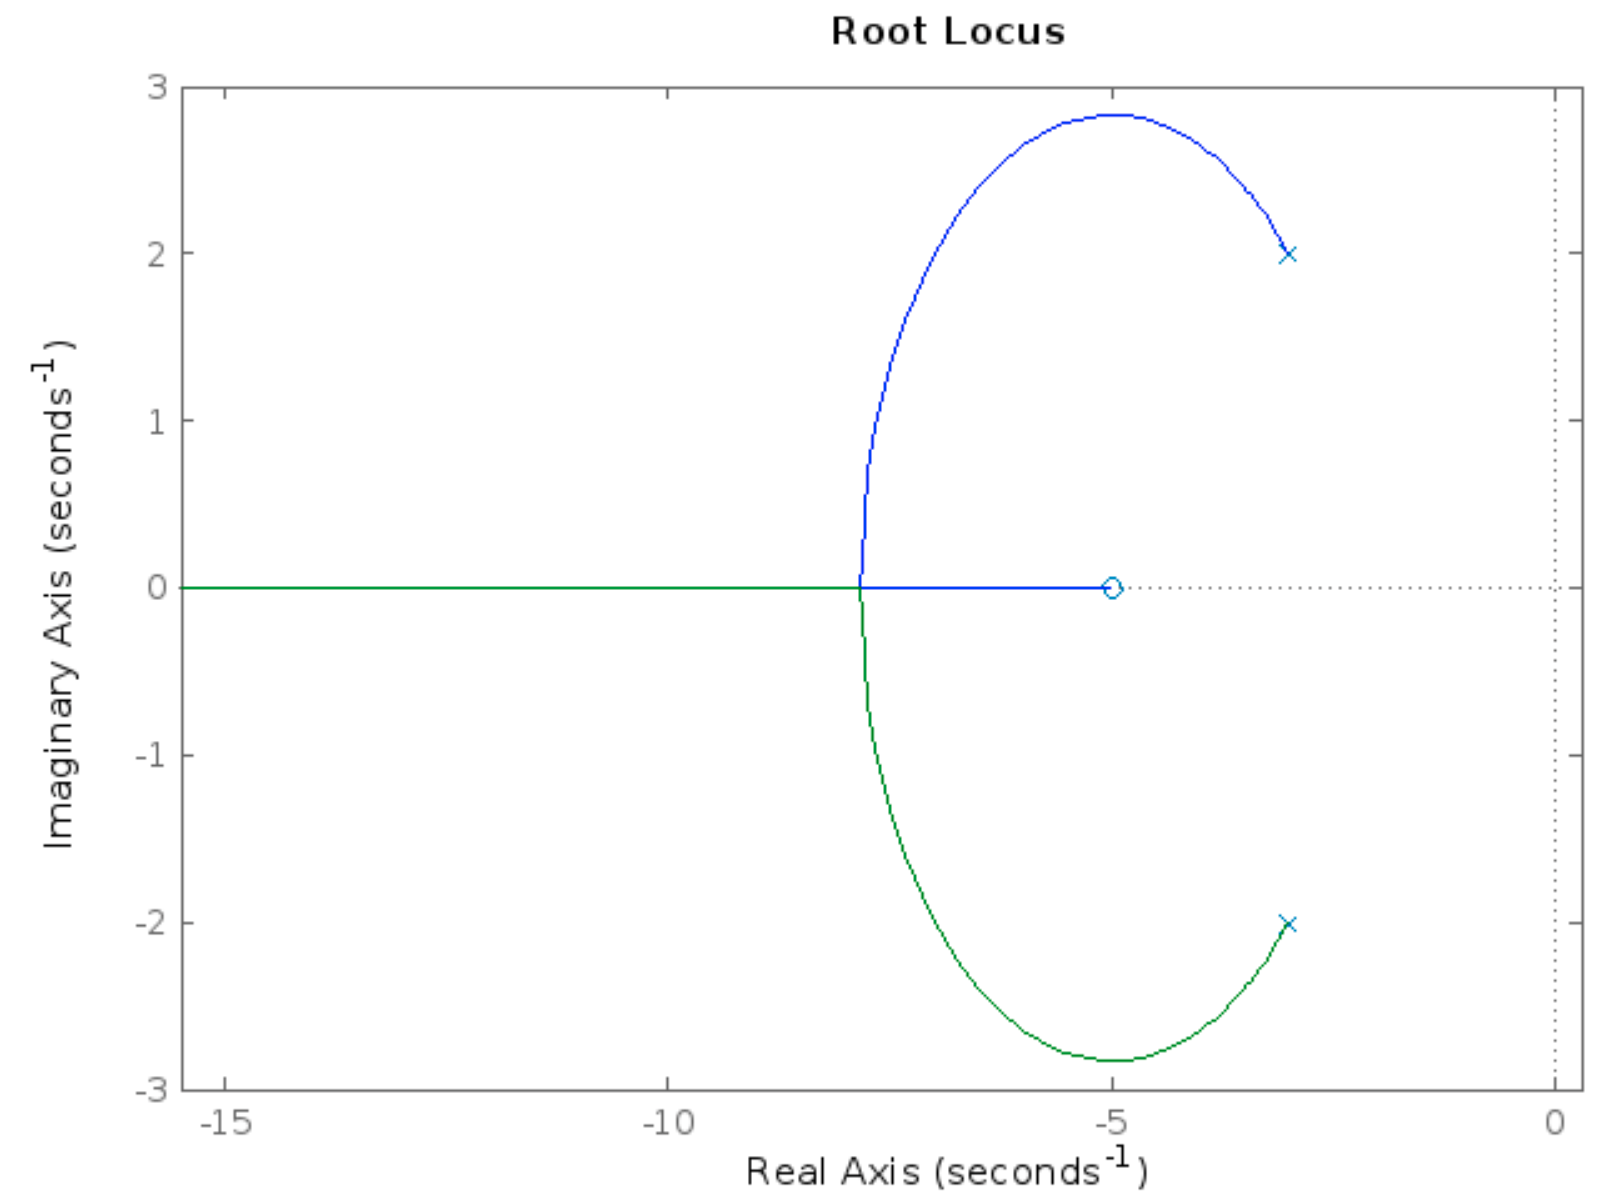
\includegraphics[scale = 0.5]{images/roo-locus1.png}
\label{filtro1}
\caption{Gráfico do Local das raízes para H^1}
\end{figure}\end{center}
\begin{matlabcode}
rlocus(1,[1 4 5])
\end{matlabcode}
\begin{center}
\begin{figure}[H]
\centering
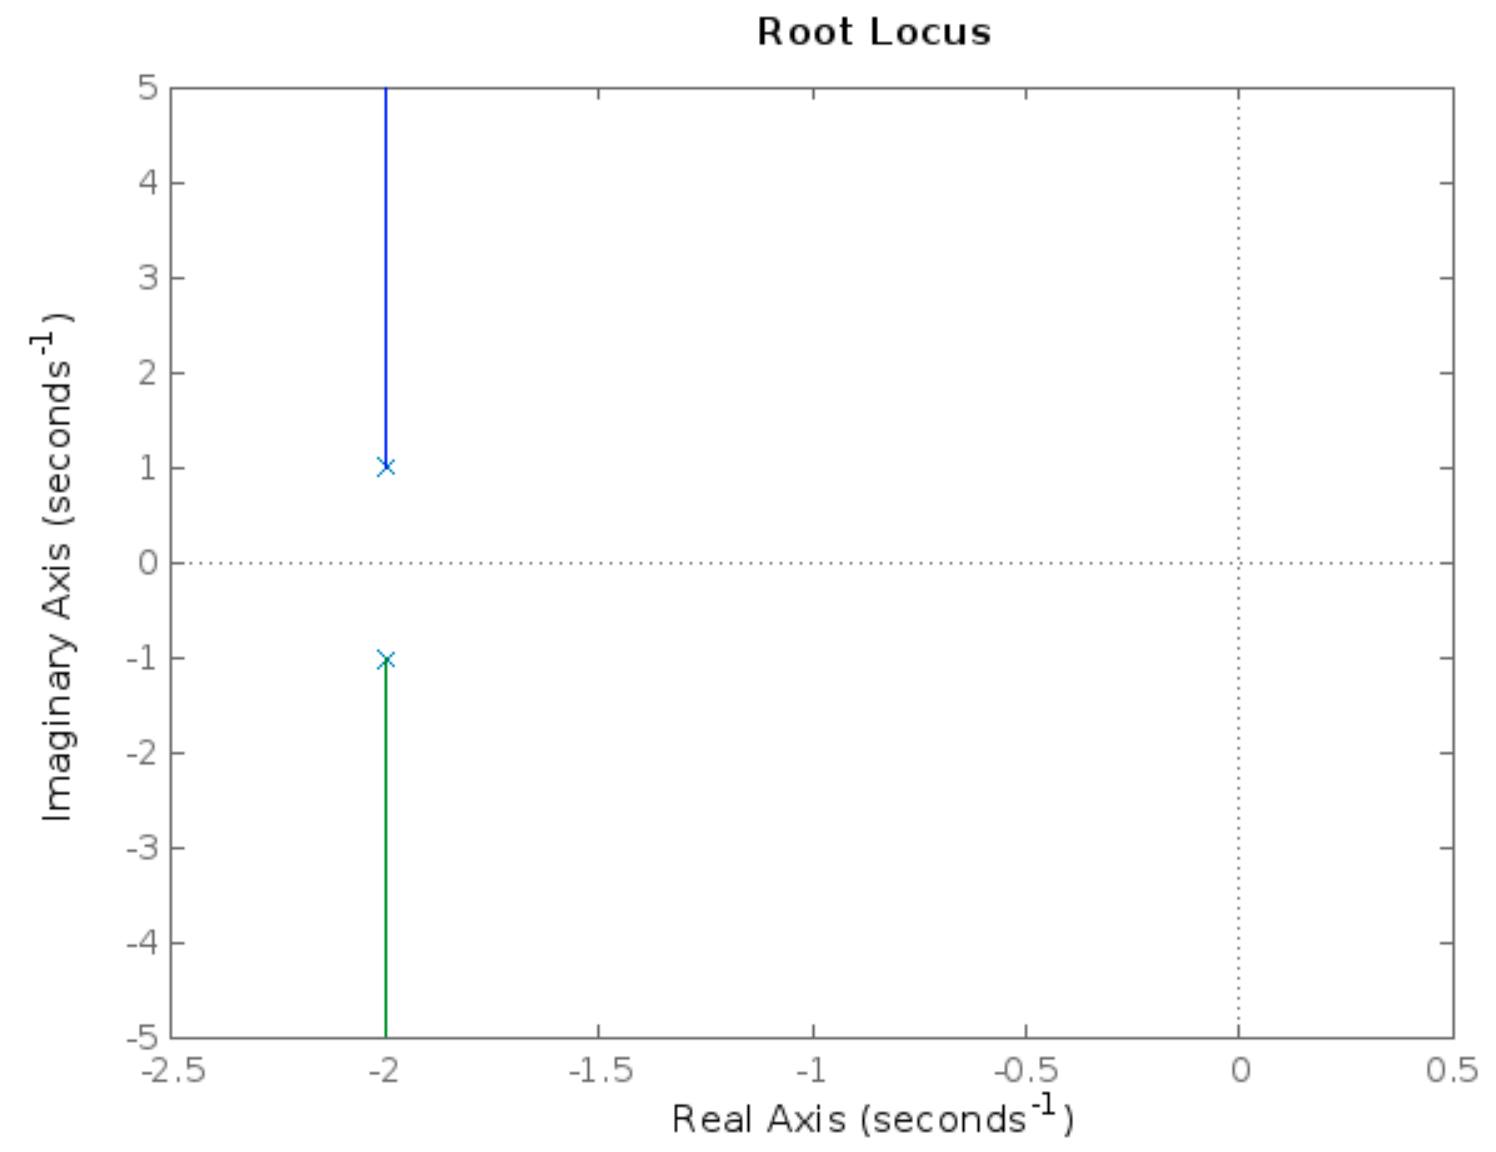
\includegraphics[scale = 0.5]{images/root-locus2.png}
\label{filtro1}
\caption{Gráfico do Local das raízes para H^2}
\end{figure}

\end{center}
\begin{matlabcode}
rlocus(H1rH2r), grid, figure();
\end{matlabcode}
\begin{center}
\begin{figure}[H]
\centering
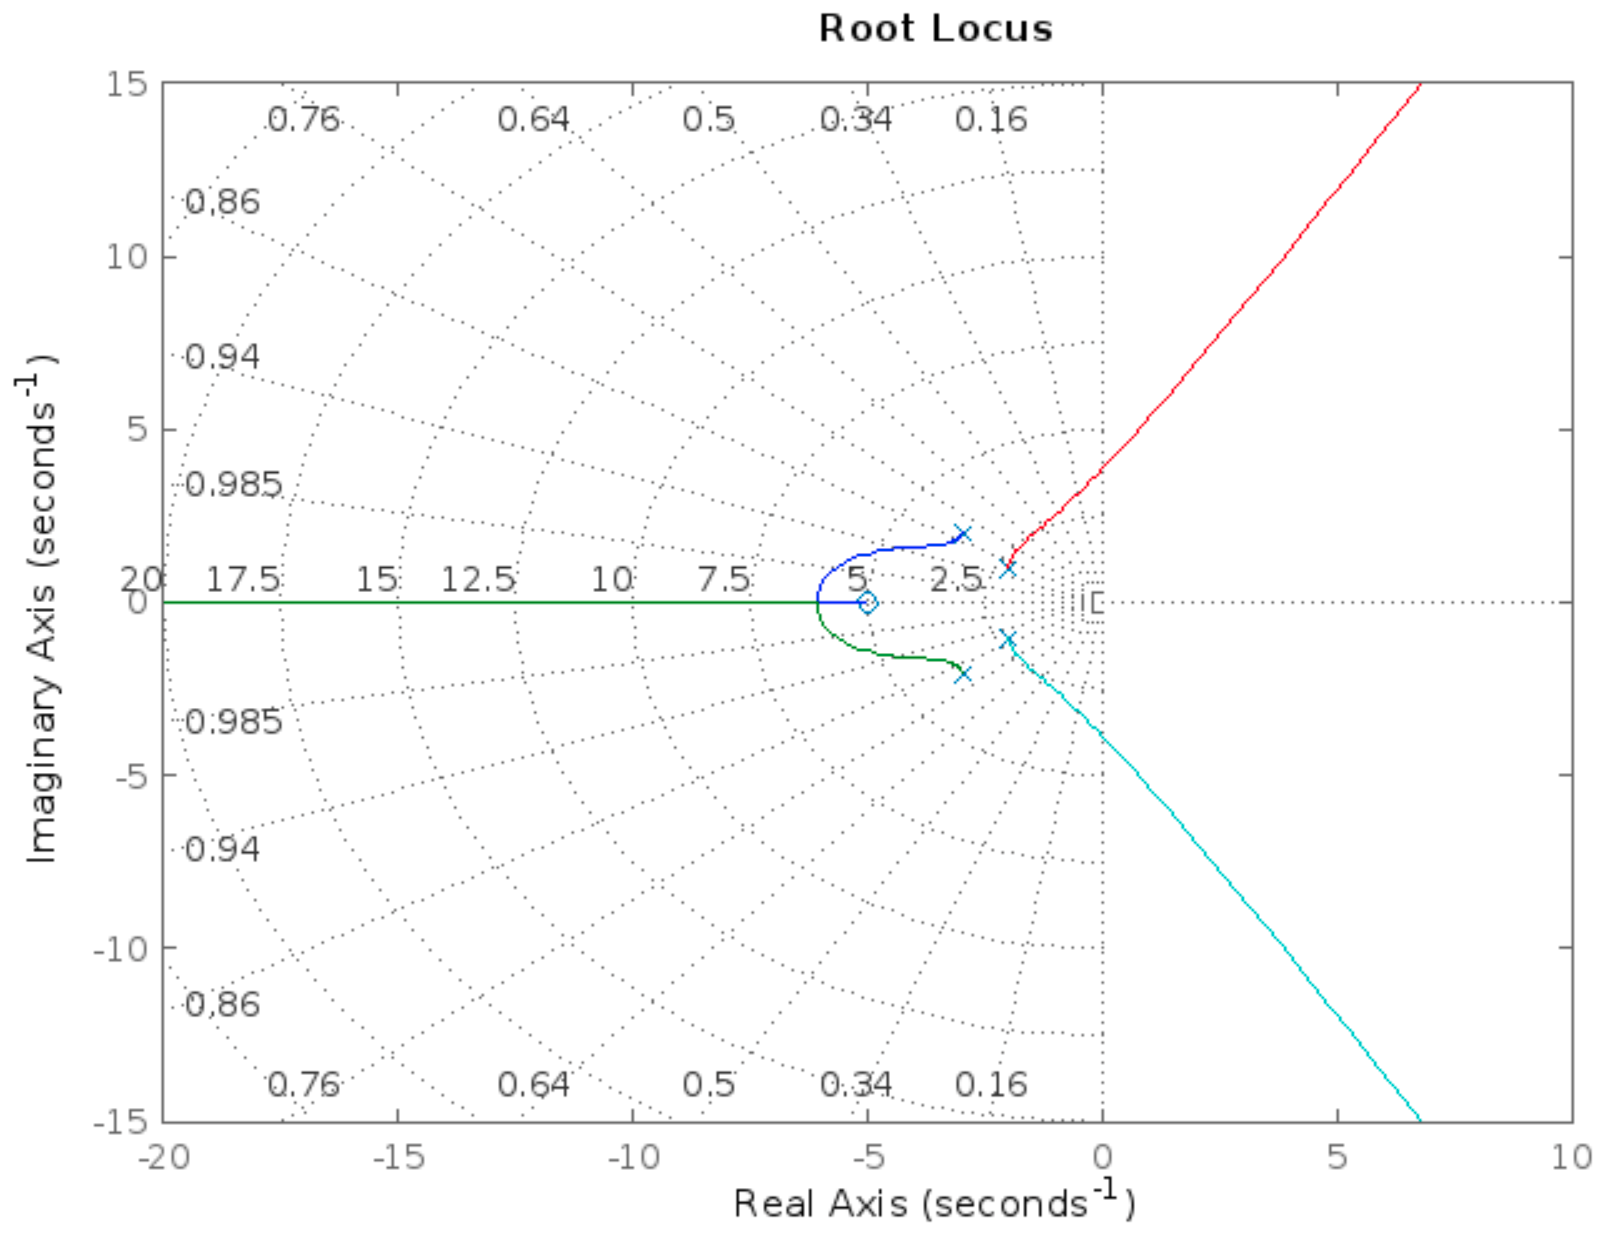
\includegraphics[scale = 0.5]{images/root-locus3.png}
\label{filtro1}
\caption{Gráfico geral do Local das raízes}
\end{figure}\end{center}



\subsection{Parte 3}
Comparar as características estabelecidas na Parte 1 com o gráfico traçado anteriormente, na parte 2.

\subsubsection{Pontos de Partida}
Onde o Lugar Geométrico das Raízes sai do eixo real e segue para o plano complexo. Ocorrem em seções do eixo real que pertencem ao Lugar das Raízes entre dois polos adjacentes.
\begin{figure}[H]
\centering
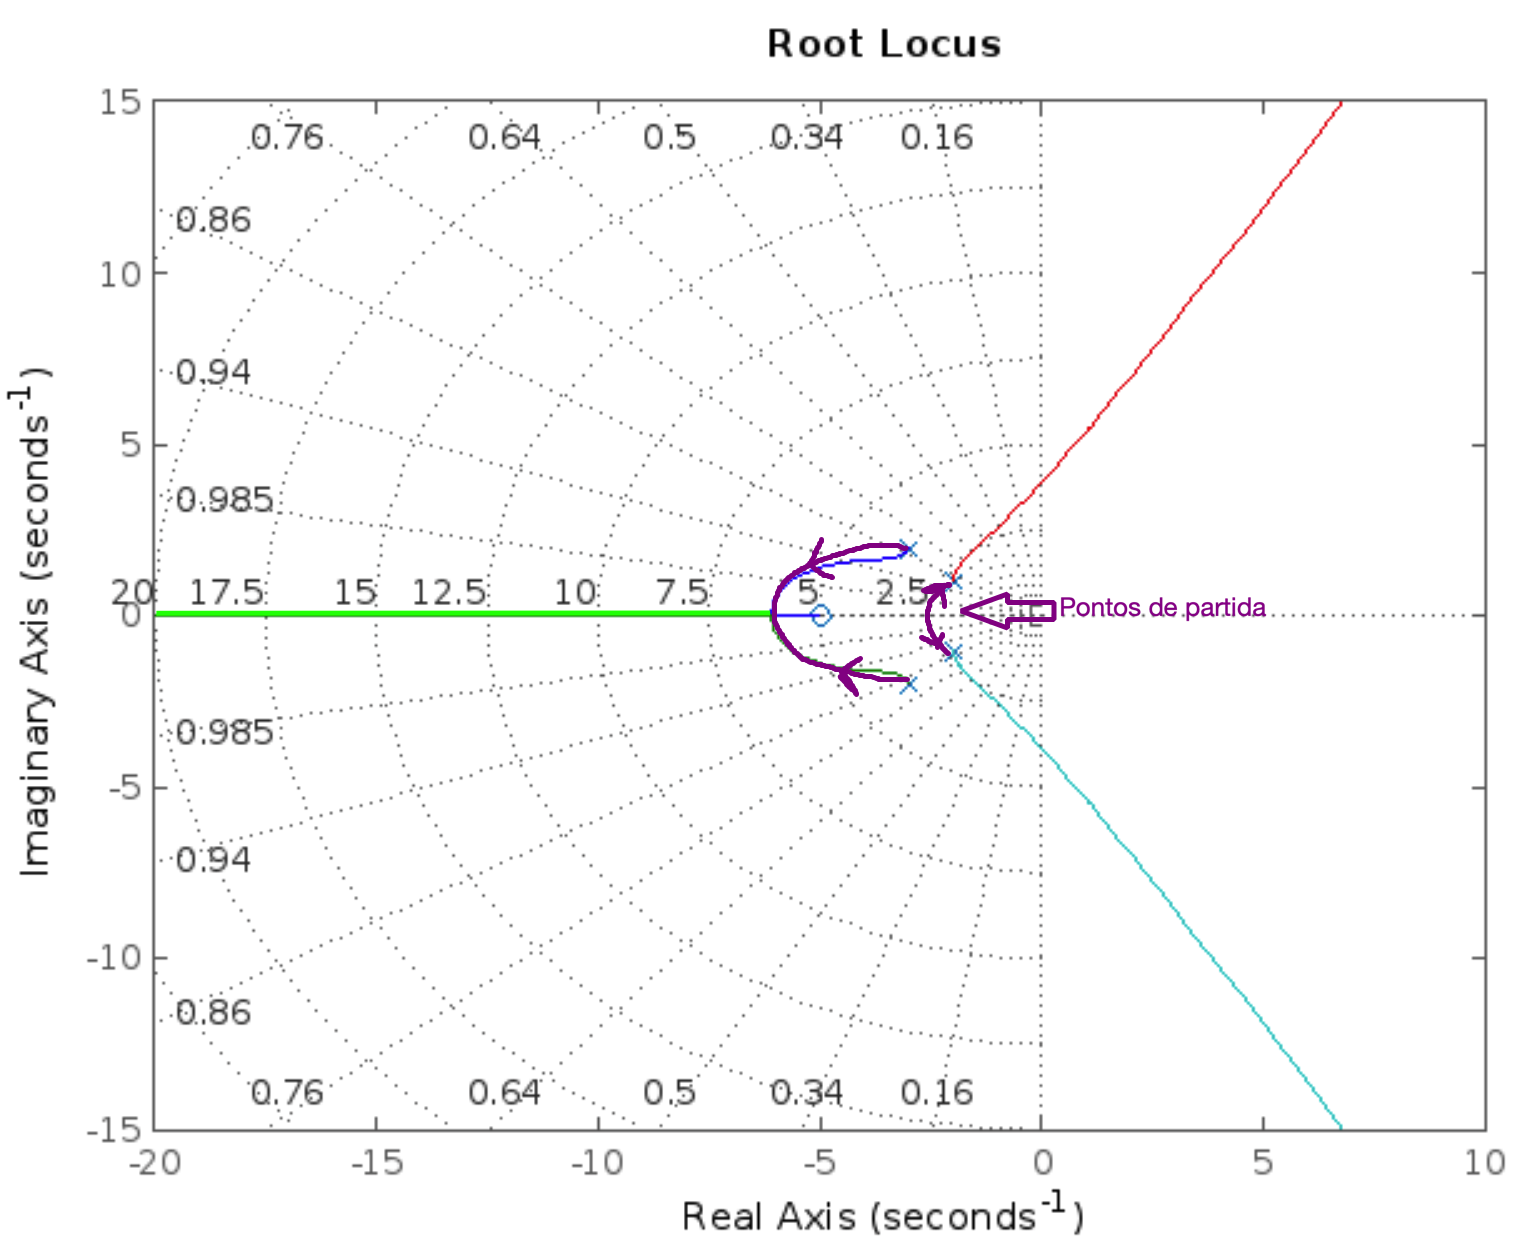
\includegraphics[scale = 0.45]{images/ptos-partida.png}
\label{filtro1}
\caption{Pontos de partida}
\end{figure}


\subsubsection{Pontos de Chegada}
Onde o Lugar Geométrico das Raízes sai do eixo complexo e segue para o plano real. Ocorrem em seções do eixo real entre dois zeros adjacentes que pertencem ao Lugar das Raízes.
\begin{figure}[H]
\centering
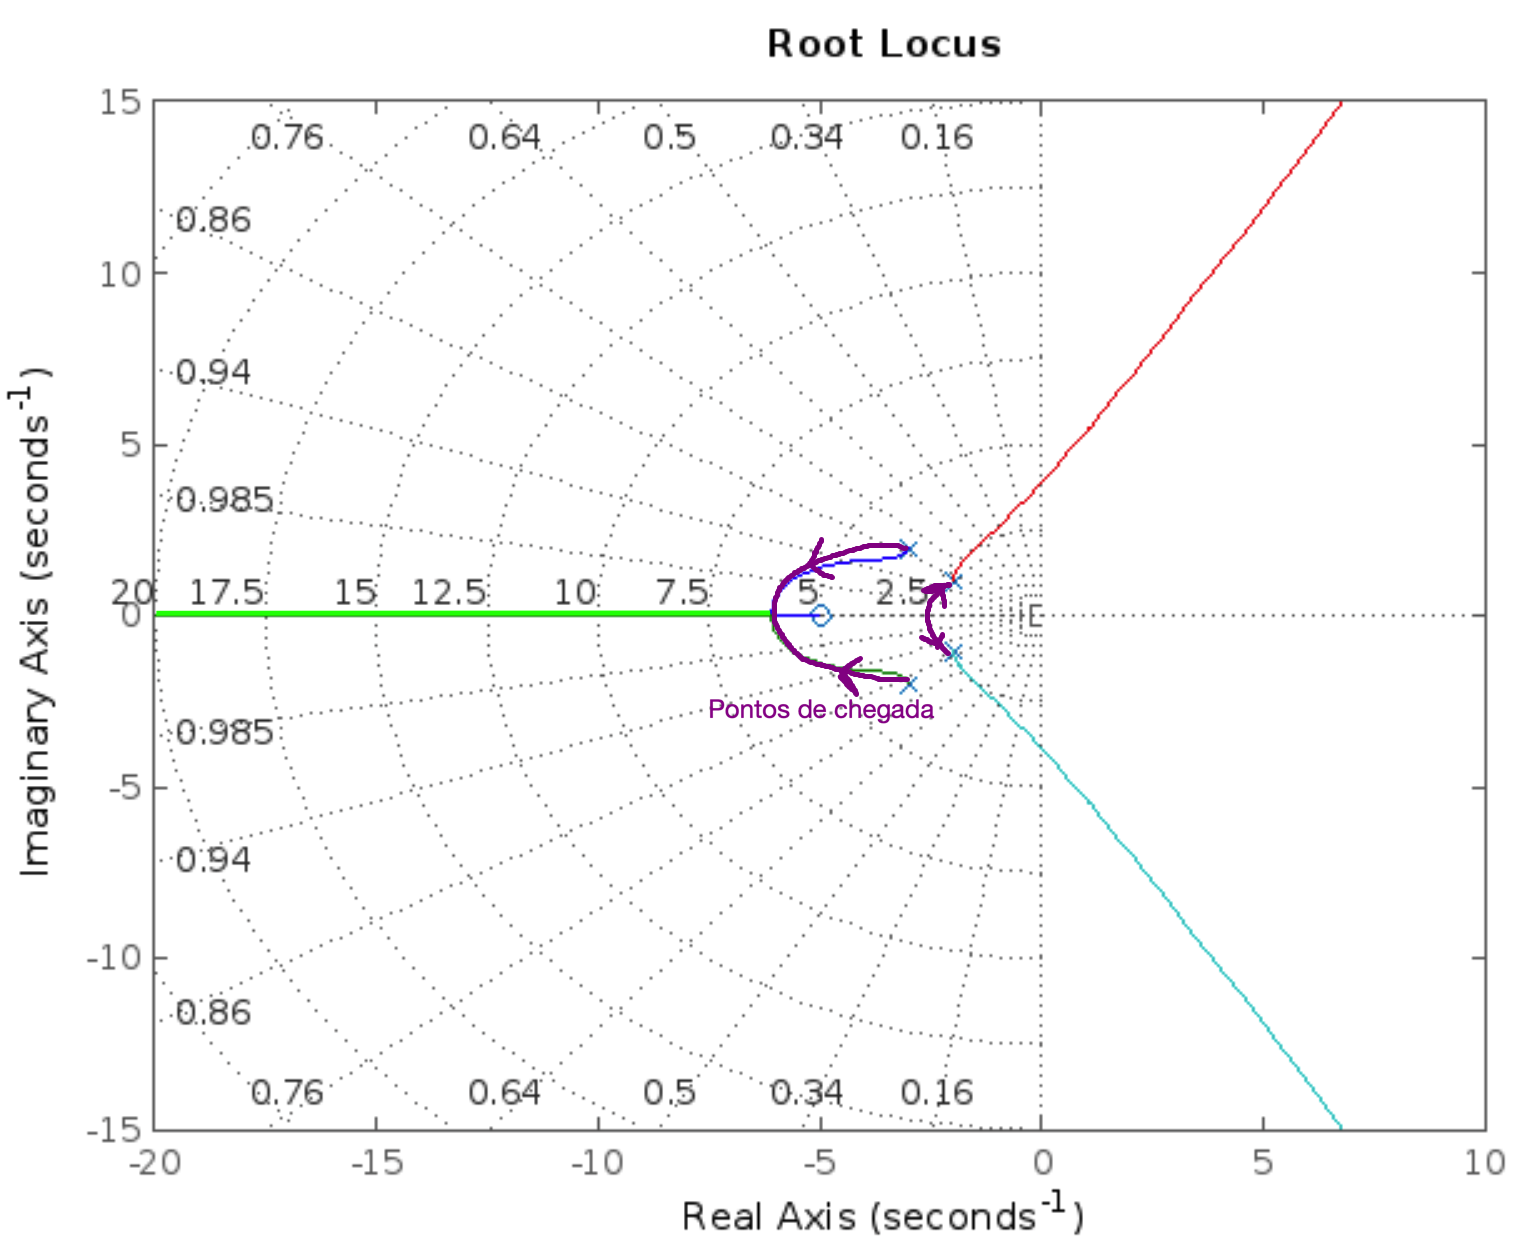
\includegraphics[scale = 0.45]{images/ptos-chegada.png}
\label{filtro1}
\caption{Pontos de chegada}
\end{figure}


\subsubsection{Características assintóticas}

\begin{figure}[H] 
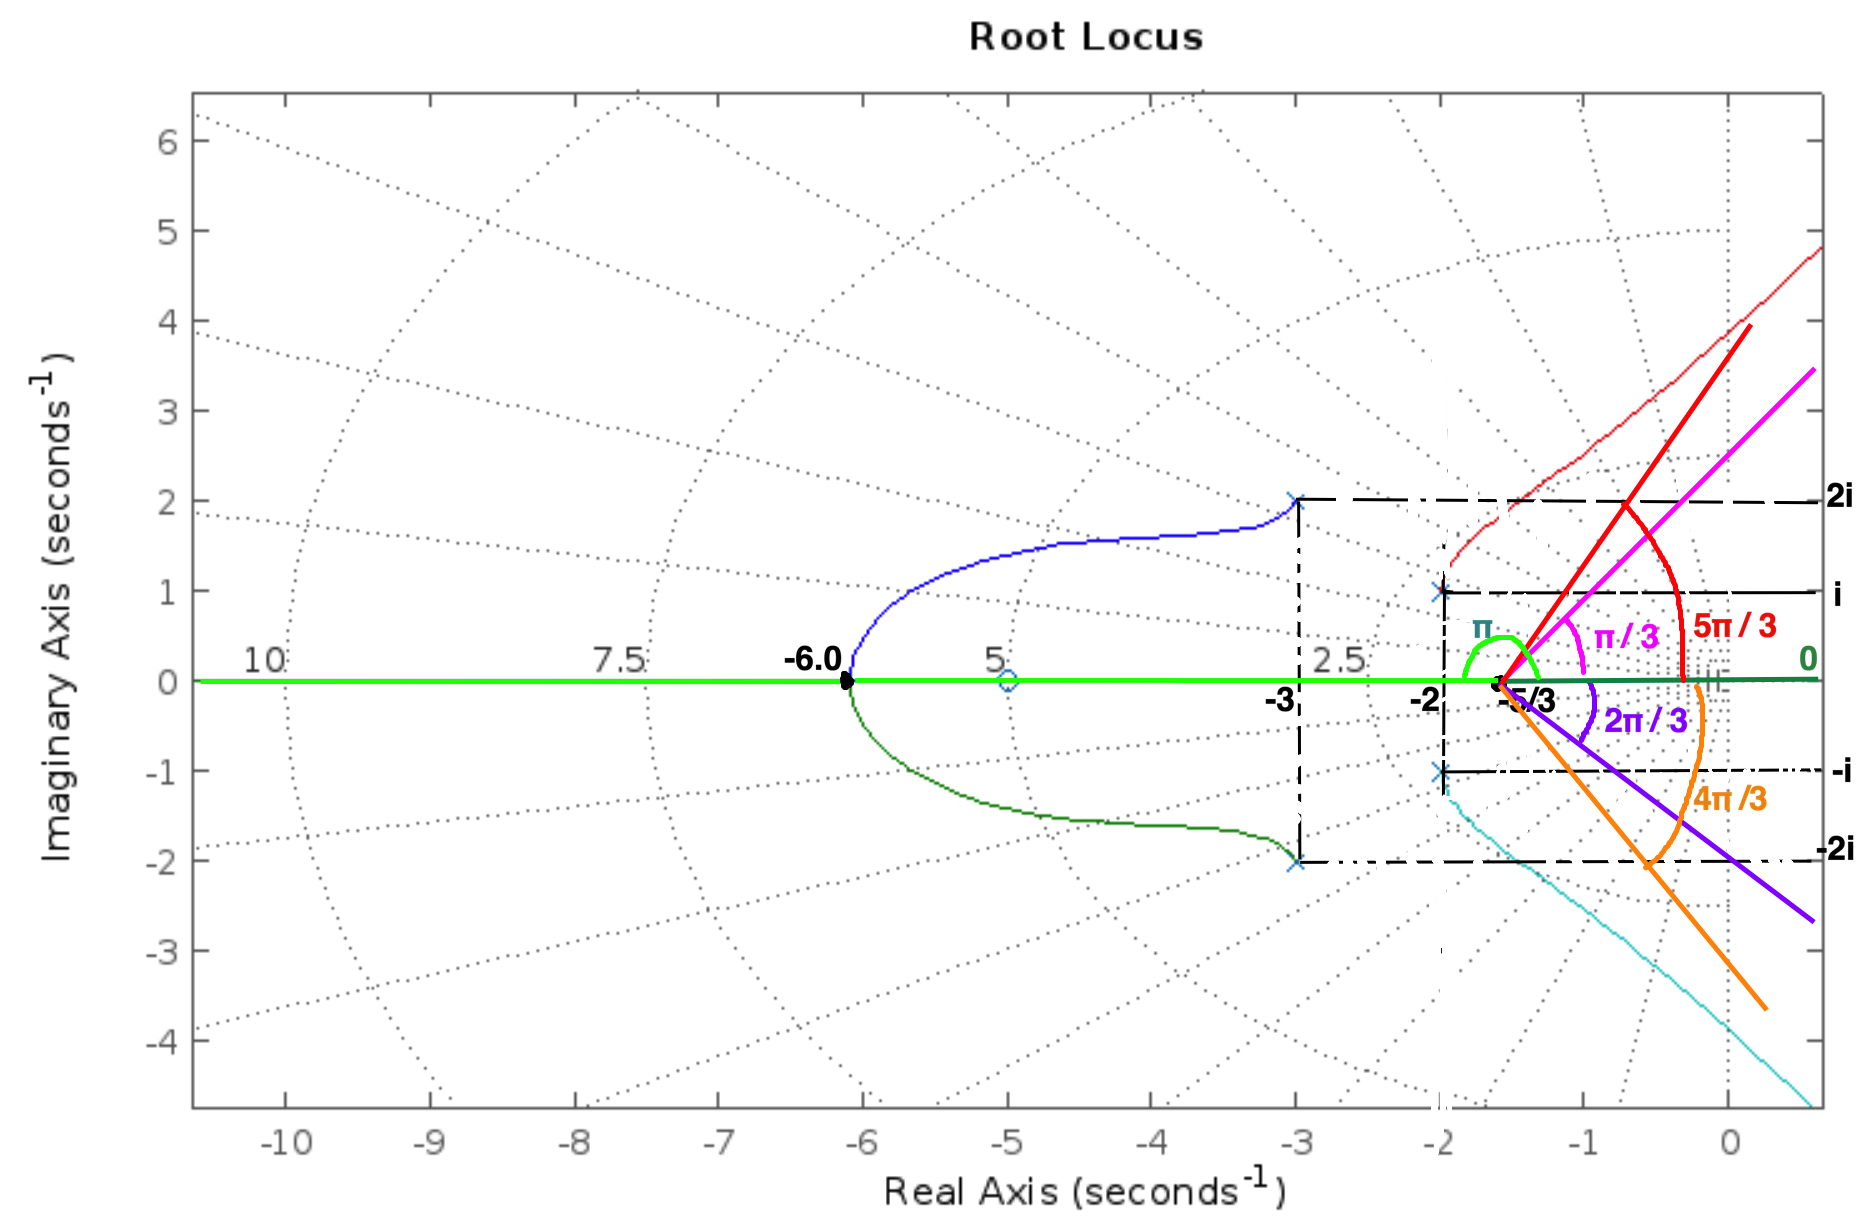
\includegraphics[scale = 0.5]{images/asympt.png}
\label{filtro1}
\caption{Assíntotas}
\end{figure}

\begin{center}
    \begin{itemize}
    \centering
    \item \color{magenta}$\theta_{01}=\frac{\pi}{3}$\color{black}; \quad \quad • \color{violet}$\theta_{02}=\frac{2\pi}{3}$\color{black};
    \item \color{green} $\theta_{11}=\pi$\color{black}; \quad \quad • \color{olive} $\theta_{12}=0$\color{black};
    \item \color{red} $\theta_{21} = \frac{5 \pi}{3}$\color{black}; \quad \quad• \color{orange}$\theta_{22} = \frac{4 \pi}{3}$\color{black};
\end{itemize}
\end{center}



\subsection{Parte 4}
Análisando do traçado, verificando se há faixas de valores de $K$ para os quais o sistema realimentado não é BIBO-estável.\\

Pelo critério de BIBO-estabilidade (\textit{Bounded Input, Bounded Output}), sabemos que:\\

• “Um sistema qualquer é estável se e somente se para toda e
qualquer entrada limitada, a saída correspondente também
for limitada”;\\
• “Um sistema linear a malha fechada, invariante no tempo, a
parâmetros parâmetros concentrados concentrados é estável estável se e somente somente se todos
os pólos de sua função de transferência de malha fechada
estão no semi-plano esquerdo aberto do plano complexo s”.

\begin{figure}[H]
\centering
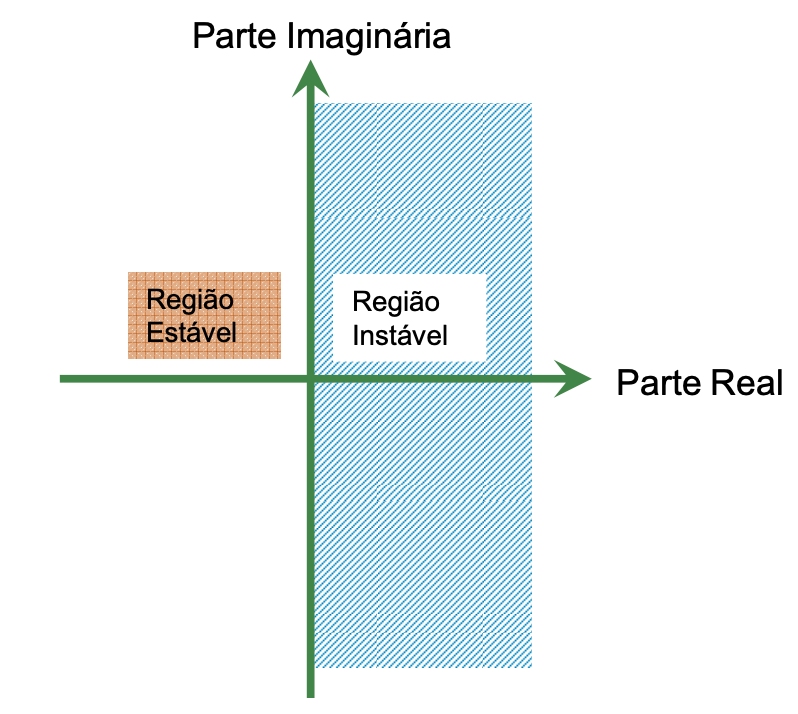
\includegraphics[scale = 0.6]{images/plano.png}
\label{filtro1}
\caption{Representação do plano com os eixos real e imaginário}
\end{figure}

Como podemos observar em (\ref{eq:polos1}) e em (\ref{eq:polos2}), uma vez que todos os polos possuem parte real negativa, temos que o sistema é estável. De acordo com (\ref{eq:estabk}), para estabilidade, $K < 74.14605\dots  $.

\newpage

% REFERENCIAS %%%%%%%%%%%%%%%%%%%%%%%%%%%%%%%%%%%%%%%%%%%%%%%%%%%%%%%%%%%%%%
    \nocite{*}
    \bibliography{src/bibliography}
    
\end{document}
\section{Referências Bibliográficas}

\end{document}